\documentclass[10pt,twocolumn,letterpaper]{article}
\usepackage[10pt,inchmargins]{sigmin}  %% template from Xi Wang.
\special{papersize=8.5in,11in}
\setlength{\pdfpagewidth}{8.5in}
\setlength{\pdfpageheight}{11in}
\usepackage[noheadfoot,
            left=1in,right=1in,top=1in,bottom=1in,
            columnsep=0.3in
            ]{geometry}
\usepackage[small,compact]{titlesec}
\usepackage[font={small,bf}]{caption}    % added 9/10/13
\usepackage[nolineno,noindent,norules]{lgrind}
\usepackage{tightenum}
\usepackage{float}
\usepackage{xspace}
\usepackage{times,pifont}
\usepackage{mathptmx}
\usepackage{subfig,graphics,graphicx,color}
\usepackage{multirow}
\usepackage{dblfloatfix} %% correctly orders single- and double-col figures
\usepackage{hyphenat}
\usepackage{mathrsfs}
\usepackage{subfig}
\usepackage{amssymb,amsmath,centernot}
\usepackage{lastpage}
\usepackage{flushend}
\usepackage{hhline}
\usepackage{authblk}
\newcommand{\doi}{10.1145/2517349.2522735}


%%% ================= START of SOSP '13 template ================= 
\makeatletter

\def\ftype@copyrightbox{8}
\def\@copyrightspace{
\@float{copyrightbox}[b]
\begin{center}
\setlength{\unitlength}{1pc}
\begin{picture}(20,6.0) 
\put(0,3){\parbox{\columnwidth}{\scriptsize

%*** SAMPLE. AUTHOR PUT SUPPLIED TEXT HERE ****

\noindent
\rule{6.0 cm}{0.2pt}\\
Permission to make digital or hard copies of part or all of this work 
for personal or classroom use is granted without fee provided that
copies are not made or distributed for profit or commercial advantage 
and that copies bear this notice and the full citation on the first
page. Copyrights for third-party components of this work must be
honored.  For all other uses, contact the Owner/Author. 

\vspace{\baselineskip}\noindent
Copyright is held by the Owner/Author(s).\\
\textit{SOSP'13}, Nov. 3--6, 2013, Farmington, Pennsylvania, USA. \\
ACM 978-1-4503-2388-8/13/11.

\noindent
http://dx.doi.org/\doi}
}
\end{picture}
\end{center}
\end@float}

\def\maketitle{\par
 \begingroup
   \def\thefootnote{\fnsymbol{footnote}}
   \def\@makefnmark{\hbox
       to 0pt{$^{\@thefnmark}$\hss}}
     \twocolumn[\@maketitle]
\@thanks
 \endgroup
 \setcounter{footnote}{0}
 \let\maketitle\relax
 \let\@maketitle\relax
 \gdef\@thanks{}\gdef\@author{}\gdef\@title{}\gdef\@subtitle{}\let\thanks\relax
 \@copyrightspace}

\makeatother

%%% ================= END of SOSP '13 template ================= 



\newcommand{\comment}[1]{}
\frenchspacing

%\doublespacing

%%%%%%%%%%%%%%%%%%%%%%%%%%%%
%     macro

\newcommand{\xxx}{\mbox{\textsc{Parrot}}\xspace}
\newcommand{\mytitle}[0]{\textbf {\xxx: A Practical Runtime \\
  for Deterministic, Stable, and Reliable Threads}}
\newcommand{\mykeywords}[0]{Deterministic Multithreading, Stable Multithreading,
  Software Model Checking, State Space Reduction}

%%%%%%%%%%%%%%%%%%%%%%%%%%%%%%%%%%%%%%%%%%%%%%%%%%%%%%%%%%%%%%%%%
% hyperref stuff

\usepackage[square,comma,numbers,sort]{natbib}
\usepackage{hypernat}
\usepackage{hyperref}

%% fill in pdf info here
\hypersetup{%
colorlinks=false,
pdfborder={0 0 0},
pdftitle={\mytitle},
pdfkeywords={\mykeywords},
bookmarksnumbered,
pdfstartview={FitH},
urlcolor=cyan,
pdfpagelabels=true,
pdfdisplaydoctitle=true,
}%

%\usepackage{breakurl}
%\usepackage[all]{hypcap}
%\renewcommand{\url}{\burl}

%%%%%%%%%%%%%%%%%%%%%%%%%%%%%%%%%%%%%%%%%%%%%%%%%%%%%%%%%%%%
% Some NICE fonts

\newfont{\BIG}{cminch}                             %--- One-inch font
\newfont{\sfbHuge}{cmssbx10 scaled\magstep5}       %-- 25pt sans serif bold
\newfont{\sfbLarger}{cmssbx10 scaled\magstep3}   %-- 12+pt sans serif boldd
\newfont{\sfblarger}{cmssbx10 scaled\magstep2}   %-- 12+pt sans serif bold
\newfont{\sfblarge}{cmssbx10 scaled\magstep1}      %-- 12pt sans serif bold
\newfont{\sfbeleven}{cmssbx10 scaled\magstephalf}  %-- 11pt sans serif bold
\newfont{\sfb}{cmssbx10}                           %-- 10pt sans serif bold
\newfont{\sfeight}{cmss8}                          %-- 8pt sans serif

%%%%%%%%%%%%%%%%%%%%%%%%
%    space tweaking

%\textwidth = 6.5 in
%\textheight = 9.0 in
%\setlength{\topmargin}{-.5in}

%\headheight = 0.0 in
%\headsep = 0.0 in
%\parskip = 0.2in
%\parindent = 0.0in

\renewcommand{\topfraction}{0.95}
\addtolength{\textfloatsep}{-0.1in}
%\addtolength{\floatsep}{0.025in}
\renewcommand\floatpagefraction{.9}
%\renewcommand\bottomfraction{.9}
\renewcommand\textfraction{.1}

\setlength{\parindent}{9pt}

% Rescue
\makeatletter
\def\v#1{{\mbox{\fontfamily{cmtt}\fontsize{\f@size}{\f@size}\selectfont #1}}}
\newcommand{\compute}{soft barrier\xspace}
\newcommand{\vcompute}{\emph{soft barrier}\xspace}
\newcommand{\computes}{soft barriers\xspace}
\newcommand{\Compute}{Soft barrier\xspace}
\newcommand{\Computes}{Soft barriers\xspace}
\newcommand{\nondet}{performance critical section\xspace}
\newcommand{\vnondet}{\emph{performance critical section}\xspace}
\newcommand{\nondets}{performance critical sections\xspace}
\newcommand{\Nondet}{Performance critical section\xspace}
\newcommand{\Nondets}{Performance critical sections\xspace}

\newcommand{\dmt}[0]{DMT\xspace}
\newcommand{\smt}[0]{StableMT\xspace}
\newcommand{\racepro}[0]{\textsc{RacePro}\xspace}
\newcommand{\tern}[0]{\textsc{Tern}\xspace}
\newcommand{\peregrine}[0]{\textsc{Peregrine}\xspace}
\newcommand{\grace}[0]{Grace\xspace}
\newcommand{\coredet}[0]{\textsc{CoreDet}\xspace}
\newcommand{\kendo}[0]{Kendo\xspace}
\newcommand{\dthreads}[0]{\textsc{DThreads}\xspace}
\newcommand{\determinator}[0]{Determinator\xspace}
\newcommand{\dbug}[0]{\textsc{dbug}\xspace}
\newcommand{\ecosys}[0]{\xxx-\dbug}

\newcommand{\apache}{\v{Apache}\xspace}
\newcommand{\ab}{\v{ApacheBench}\xspace}
\newcommand{\mysql}{\v{MySQL}\xspace}
\newcommand{\sysbench}{\v{SysBench}\xspace}
\newcommand{\mplayer}[0]{{MPlayer}\xspace}
\newcommand{\mencoder}[0]{\v{mencoder}\xspace}
\newcommand{\pbzip}[0]{\v{PBZip2}\xspace}
\newcommand{\aget}[0]{\v{aget}\xspace}
\newcommand{\mongoose}[0]{\v{Mongoose}\xspace}
\newcommand{\pfscan}[0]{\v{pfscan}\xspace}
\newcommand{\fft}[0]{\v{fft}\xspace}
\newcommand{\luc}[0]{\v{lu\_cb}\xspace}
\newcommand{\lun}[0]{\v{lu\_ncb}\xspace}
\newcommand{\barnes}[0]{\v{barnes}\xspace}
\newcommand{\radix}[0]{\v{radix}\xspace}
\newcommand{\radiosity}[0]{\v{radiosity}\xspace}
\newcommand{\waters}[0]{\v{water-spatial}\xspace}
\newcommand{\watern}[0]{\v{water-nsquared}\xspace}
\newcommand{\oceanncp}[0]{\v{ocean}\xspace}
\newcommand{\oceancp}[0]{\v{ocean}\xspace}
\newcommand{\fmm}[0]{\v{fmm}\xspace}
\newcommand{\volrend}[0]{\v{volrend}\xspace}
\newcommand{\cholesky}[0]{\v{cholesky}\xspace}
\newcommand{\streamcluster}[0]{\v{streamcluster}\xspace}
\newcommand{\blackscholes}[0]{\v{blackscholes}\xspace}
\newcommand{\swaptions}[0]{\v{swaptions}\xspace}
\newcommand{\bodytrack}[0]{\v{bodytrack}\xspace}
\newcommand{\bodytrackopenmp}[0]{\v{bodytrack-openmp}\xspace}
\newcommand{\ferret}[0]{\v{ferret}\xspace}
\newcommand{\dedup}[0]{\v{dedup}\xspace}
\newcommand{\raytrace}[0]{\v{raytrace}\xspace}
\newcommand{\canneal}[0]{\v{canneal}\xspace}
\newcommand{\racey}[0]{\v{racey}\xspace}
\newcommand{\freqmine}[0]{\v{freqmine}\xspace}
\newcommand{\vips}[0]{\v{vips}\xspace}
\newcommand{\xtwosixfour}[0]{\v{x264}\xspace}
\newcommand{\fluidanimate}[0]{\v{fluidanimate}\xspace}
\newcommand{\facesim}[0]{\v{facesim}\xspace}
\newcommand{\rtviewraytrace}[0]{\v{rtview\_raytrace}\xspace}
\newcommand{\wordcount}[0]{\v{word\_count}\xspace}
\newcommand{\klee}[0]{\textsc{klee}\xspace}
\newcommand{\woodpecker}[0]{\textsc{woodpecker}\xspace}
\newcommand{\splashx}[0]{\mbox{SPLASH-2x}\xspace}
\newcommand{\parsec}[0]{\mbox{PARSEC}\xspace}
\newcommand{\phoenix}[0]{\mbox{Phoenix}\xspace}
\newcommand{\pthread}[0]{\mbox{Pthreads}\xspace}

\newcommand{\kmeans}[0]{\v{kmeans}\xspace}
\newcommand{\kmeanspthread}[0]{\v{kmeans-pthread}\xspace}
\newcommand{\linearregre}[0]{\v{linear-regression}\xspace}
\newcommand{\linearregrepthread}[0]{\v{linear-regression-pthread}\xspace}
\newcommand{\matrixmult}[0]{\v{matrix-multiply}\xspace}
\newcommand{\matrixmultpthread}[0]{\v{matrix-multiply-pthread}\xspace}
\newcommand{\wordcnt}[0]{\v{word-count}\xspace}
\newcommand{\wordcntpthread}[0]{\v{word-count-pthread}\xspace}
\newcommand{\stringmatch}[0]{\v{string-match}\xspace}
\newcommand{\stringmatchpthread}[0]{\v{string-match-pthread}\xspace}
\newcommand{\histogram}[0]{\v{histogram}\xspace}
\newcommand{\histogrampthread}[0]{\v{histogram-pthread}\xspace}
\newcommand{\pca}[0]{\v{pca}\xspace}
\newcommand{\pcapthread}[0]{\v{pca-pthread}\xspace}

\newcommand{\partition}[0]{\mbox{\v{partition}}\xspace}
\newcommand{\nthelement}[0]{\mbox{\v{nth\_element}}\xspace}
\newcommand{\partialsort}[0]{\mbox{\v{partial\_sort}}\xspace}
\newcommand{\ua}[0]{\v{ua}\xspace}
\newcommand{\is}[0]{\v{is}\xspace}
\newcommand{\npb}[0]{\mbox{NPB}\xspace}
\newcommand{\imagick}[0]{\mbox{ImageMagick}\xspace}
\newcommand{\openldap}[0]{{OpenLDAP}\xspace}
\newcommand{\redis}[0]{{Redis}\xspace}
\newcommand{\bdb}[0]{{Berkeley DB}\xspace}
\newcommand{\openmp}[0]{{OpenMP}\xspace}
\newcommand{\libgomp}[0]{\v{libgomp}\xspace}
\newcommand{\vtune}[0]{\v{VTune}\xspace}

%% imagick programs
\newcommand{\convertshear}[0]{\v{convert\_shear}\xspace}
\newcommand{\montage}[0]{\v{montage}\xspace}

\newcommand{\nprog}[0]{108\xspace}
\newcommand{\nrealprog}[0]{55\xspace}
\newcommand{\nstl}[0]{33\xspace}
\newcommand{\nimagick}[0]{14\xspace}
\newcommand{\nparsec}[0]{15\xspace}
\newcommand{\nphoenix}[0]{14\xspace}
\newcommand{\nsplash}[0]{14\xspace}
\newcommand{\nnpb}[0]{10\xspace}
\newcommand{\nbenchmarks}[0]{53\xspace}
\newcommand{\ndatapartition}[0]{86\xspace}
\newcommand{\nprogadhocsync}[0]{5\xspace}
\newcommand{\nprogtimeout}[0]{5\xspace}

\newcommand{\nprognohints}[0]{18\xspace}
\newcommand{\nprogneedhints}[0]{90\xspace}
\newcommand{\nprognondethints}[0]{9\xspace}
\newcommand{\nprognondetandnetwork}[0]{11\xspace} % the UA program is excluded.
\newcommand{\nprognonondethints}[0]{99\xspace}
\newcommand{\nproglineuphints}[0]{81\xspace}
\newcommand{\nproggenericlineuphints}[0]{43\xspace}
\newcommand{\nprogspecificlineuphints}[0]{38\xspace}
\newcommand{\nlineofhints}[0]{109\xspace}
\newcommand{\nlineofcomputehints}[0]{87\xspace}
\newcommand{\nlineofnondethints}[0]{22\xspace}
\newcommand{\hintsperprog}[0]{1.2\xspace}
\newcommand{\nlineupfails}[0]{12\xspace}

%% effects of perfomance hints.
\newcommand{\genericnolineup}[0]{500\%\xspace}
\newcommand{\genericlineup}[0]{0.8\%\xspace}
\newcommand{\specificnolineup}[0]{460\%\xspace}
\newcommand{\specificlineup}[0]{19.1\%\xspace}
\newcommand{\nondetnohints}[0]{830\%\xspace}
\newcommand{\nondethints}[0]{42.1\%\xspace}
\newcommand{\overallnohints}[0]{510\%\xspace}
\newcommand{\overallhints}[0]{11.9\%\xspace}

%% our geometric mean overhead on standard workload.
\newcommand{\meanoverhead}[0]{12.7\%\xspace}
\newcommand{\meanrealoverhead}[0]{6.9\%\xspace}
\newcommand{\meanbenchoverhead}[0]{19.0\%\xspace}

%% model checking reduction.
%% nprogshrink, totally 56: 50 programs with out nondet hints, and 6 programs with network or nondet hints.
\newcommand{\shrinkscale}[0]{$10^{6}$--$10^{19734}$\xspace}
\newcommand{\nprogshrink}[0]{56\xspace}
\newcommand{\nprognondetshrink}[0]{5\xspace}
\newcommand{\nprogverifiedxxx}[0]{99\xspace}
\newcommand{\nprogverifieddbug}[0]{43\xspace}

%% overheads in comparison table.
\newcommand{\nprogcompared}[0]{25\xspace}
\newcommand{\xxxcompoverhead}[0]{11.8\%\xspace}
\newcommand{\dthreadssyncoverhead}[0]{150.0\%\xspace}
\newcommand{\dthreadssyncoverheadnoflui}[0]{112.5\%\xspace}
%\newcommand{\dthreadsoverhead}[0]{1,173\%\xspace}
\newcommand{\dthreadsexampleoverhead}[0]{7.7$\times$\xspace}
\newcommand{\coredetoverhead}[0]{115.1\%\xspace}
\newcommand{\overeach}[0]{10$\times$\xspace}
\newcommand{\overcombined}[0]{4$\times$\xspace}

%% should not use these any more.
\newcommand{\overcoredet}[0]{20.7\xspace}
\newcommand{\overdthreadssync}[0]{131.3\xspace}
\newcommand{\overdthreadsfull}[0]{47.3\xspace}

\newcommand{\npthreadsync}[0]{38\xspace}
\newcommand{\nioync}[0]{33\xspace}
\newcommand{\locsmcmc}[0]{243\xspace}

\newcommand{\eg}{{e.g.}}
\newcommand{\ie}{{i.e.}}
\newcommand{\etc}{{etc}}
\newcommand{\para}[1]{\vspace{.00in}\noindent{\bf #1}}
\newcommand{\wrt}{{w.r.t. }}
\newcommand{\cf}{{cf. }}

\newcommand{\github}[0]{\url{github.com/columbia/smt-mc}}

\def\LGfsize{\footnotesize}
\pagestyle{empty}

\begin{document}

% Hack for: Package caption Error: No float type 'copyrightbox' defined.
\newcounter{copyrightbox}

\date{}

\title{\mytitle}

\author[+]{\hspace{0 mm}\fontsize{10}{10}\selectfont Heming Cui}
\author[*]{Jiri Simsa}
\author[+]{Yi-Hong Lin}
\author[+]{Hao Li}
\author[*]{Ben Blum}
\author[+]{Xinan Xu}
\author[+]{\\\hspace{0 mm}\fontsize{10}{10}\selectfont Junfeng Yang}
\author[*]{Garth A. Gibson}
\author[*]{Randal E. Bryant\vspace{-3.0 mm}}
\setlength{\affilsep}{1em}
\renewcommand\AB@affilsepx{\hspace{28.0 mm}\protect\Affilfont}
%\affil[+]{Department of Computer Science}
%\renewcommand\AB@affilsepx{\\\protect\Affilfont}
%\affil[*]{Department of Computer Science\hspace{1.0mm}}
\affil[+]{\textrm\fontsize{10}{10}\selectfont Columbia University}
\affil[*]{\textrm Carnegie Mellon University\vspace{-7.0 mm}}
%\affil[ ]{\textrm{\small {\hspace{-8.5 mm}\{heming, yl2790, lihao, xx2153, junfeng\}@cs.columbia.edu
%  \hspace{15 mm}\{jsimsa, bblum, garth, randy.bryant\}@cs.cmu.edu}}}
\maketitle
\thispagestyle{empty}

\begin{sloppypar}
\begin{abstract}
Multithreaded programs are notoriously hard to get right, and a key reason is:
these programs have \emph{too many} possible thread interleavings (or
schedules) at runtime. It is extremely challenging for existing techniques to
test, analyze, or verify all these schedules, making multithreaded programs
prone to various reliability and security bugs. This article introduces
 Stable multithreading (\smt), a new idea that can greatly
 reduce the number of possible schedules for multi-threaded programs on all
 inputs with reasonable performance overhead, making
 these programs much easier to get right. This article also presents three
 \smt software systems, \tern, \peregrine, and \parrot, with each addressing
 distinct research challenges. To show that \smt can greatly improve software
 reliability and security, this article describes two promising applications of \smt:
 (1) greatly improving schedule coverage of a popular systematic testing technique
 called model checking, and  (2) enabling transparent state-machine replication for multi-threaded programs.

\end{abstract}
\end{sloppypar}

\begin{sloppypar}
%% %\category{D.2.5}{Software Engineering}{Testing and Debugging}
%% \category{D.4.5}{Operating Systems}{Threads, Reliability}
%% \category{D.2.4}{Software Engineering}{Software/Program Verification}
%% \terms{Algorithms, Design, Reliability, Performance}
%% \keywords{\mykeywords}

%% \vskip 2mm
%% \noindent {\small \bf Categories and Subject Descriptors:} \vskip -.2mm
%% \noindent
%% {\footnotesize D.4.5~[{\bf Operating Systems}]: {Threads, Reliability}\\
%% D.2.4~[{\bf Software Engineering}]: {Software/Program Verification};}
%% \vskip 1mm
%% \noindent {\small \bf General Terms:} \vskip -.2mm
%% \noindent
%% {\footnotesize Algorithms, Design, Reliability, Performance}
%% \vskip 1mm
%% \noindent {\small \bf Keywords:} \vskip -.2mm
%% \noindent
%% {\footnotesize \mykeywords}

\vskip 2mm
\noindent {\small \bf Categories and Subject Descriptors:}
{\small D.4.5~[{\bf Operating Systems}]: {Threads, Reliability};
  D.2.4~[{\bf Software Engineering}]: {Software/Program Verification};}
\vskip .1mm
\noindent {\small \bf General Terms:} {\small Algorithms, Design,
  Reliability, Performance}
\vskip .1mm
\noindent {\small \bf Keywords:} {\small \mykeywords}

\end{sloppypar}

\begin{sloppypar}

\section{Introduction} \label{sec:intro}

Multithreaded programs are difficult to write, test, and debug.  A key
reason is nondeterminism: different runs of a multithreaded
program may show different behaviors, depending on how the threads
interleave~\cite{lee06}.
% We term the interleaved executions of threads a schedule.

Two main factors make threads interleave nondeterministically.  The first
is \emph{scheduling}, how the OS and hardware schedule threads.
Scheduling nondeterminism is not essential and can be eliminated without
affecting correctness for most programs.  The second is \emph{input}, what
data (\emph{input data}) arrives at what time (\emph{input timing}).
% (\eg, when a \v{recv()} call returns).
Input nondeterminism sometimes is essential because major changes in
inputs require different schedules.  However, frequently input
nondeterminism is not essential and the same schedule can be used to
process many different inputs (\S\ref{sec:define-schedule}).  We believe
nonessential nondeterminism should be eliminated in favor of determinism.

% Scheduling nondeterminism is unique to multithreaded programs.  

% Input nondeterminism affects both, but has a unique effect on
% multithreaded programs: make threads interleave differently.  

% for example, pbzip2 
%   compressing and decompressing, 
%   same file blocks

\emph{Deterministic multithreading} (\dmt)
systems~\cite{dmp:asplos09,coredet:asplos10,kendo:asplos09} make threads
more deterministic by eliminating scheduling nondeterminism.
Specifically, they constrain a multithreaded program such that it always
uses the same thread schedule for the same input.  By doing so, these
systems make program behaviors repeatable, increase testing confidence,
and ease bug reproduction.
% \dmt is different from deterministic replay~\cite{r2:osdi, friday2007,
% srinivasan:flashback, revirt, dejavu, vmware-record-replay,
% smp-revirt:vee08, pres:sosp09, scribe:sigmetrics10, odr:sosp09,
% capo:asplos09}, a bug-reproducing technique that often passively records
% execution (\eg, memory accesses/thread schedules) instead of actively
% constraining it.

Unfortunately, though existing \dmt systems eliminate scheduling
nondeterminism, they do not reduce input nondeterminism.  In fact, they
may aggravate the effects of input nondeterminism because of their design
limitation: when scheduling the threads to process an input, they consider
only this input and ignore previous similar inputs.  This stateless design
makes schedules over-dependent on inputs, so that a slight change to
inputs may force a program to (ad)venture into a vastly different,
potentially buggy schedule, defeating many benefits of determinism.  We
call this the \emph{instability} problem. 
This problem is confirmed by our results (\S\ref{sec:bug-stable}) from
an existing \dmt system~\cite{coredet:asplos10}.

In fact, even with the same input, existing \dmt systems may still force a
program into different schedules for minor changes in the execution
environment such as processor type and shared library.  Thus,
developers may no longer be able to reproduce bugs by running their
program on the bug-inducing input, because their machine may differ from
the machine where the bug occurred.

This paper presents \tern, a schedule-centric, stateful \dmt system.  It
addresses the instability problem using an idea called \emph{schedule
  memoization} that memoizes past working schedules and reuses them for
future inputs.  Specifically, \tern maintains a cache of past schedules and
the input constraints required to reuse these schedules.  When an input arrives,
\tern checks the input against the memoized constraints for a compatible
schedule.  If it finds one, it simply runs the program while enforcing
this schedule.  Otherwise, it runs the program to memoize a schedule and
the input constraints of this schedule for future reuse.  By reusing
schedules, \tern avoids potential errors in unknown schedules.  This
advantage is illustrated in Figure~\ref{fig:idea}.

%   \tern thus achieves stability because many programs frequently reuse
%   schedules ().

A real-world analogy to schedule memoization is the natural tendencies in
humans and animals to follow familiar routes to avoid possible hazards
along unknown routes.  Migrant birds, for example, often migrate along
fixed ``flyways.''  We thus name our system after the Arctic Tern, a bird
species that migrates the farthest among all migrants~\cite{artic-tern-wiki}.  

A second advantage of schedule memoization is that it makes schedules
explicit, providing flexibility in deciding when to memoize certain
schedules.  For instance, \tern allows developers to populate a schedule
cache offline, to avoid the overhead of doing so online.  Moreover,
\tern can check for errors (\eg, races) in schedules and memoize only the
correct ones, thus avoiding the buggy schedules and amortizing the
cost of checking for errors.

To make \tern practical, it must handle server programs which frequently
use threads for performance.  These programs present two challenges for
\tern: (1) they often process client inputs (requests) as they arrive, thus
suffering from input timing nondeterminism, which existing \dmt systems do
not handle and (2) they may run continuously, making their schedules
effectively infinite and too specific to reuse.

\tern addresses these challenges using a simple idea called
\emph{windowing}.  Our insight is that server programs tend to return to the
same quiescent states.
% are done processing a batch of inputs.  Based on this insight,
Thus, \tern splits the continuous request stream of a server into
\emph{windows} and lets the server quiesce in between, so that \tern can
memoize and reuse schedules across windows.  Within a window, it admits
requests only at fixed schedule points, reducing timing nondeterminism.

% effectively turns server programs into ``batch programs.''  
% Based on this observation, \tern breaks continuous request streams into
% windows and let the server program quiesces between two windows.
%% Instead of processing the inputs as they arrive, \tern buffers the inputs
%% in a fix-sized window.  When the window is full or no new inputs arrive
%% for a period of time, \tern processes the (possibly partial) window of
%% uncorrelated inputs all together.  \tern waits for the current window to be
%% fully processed before it moves onto the next window to avoid interference
%% between windows.
%% % isolates windows from each other so that they do not interfere.
%% \tern memoizes the aggregate schedule of a window and later uses it on
%% other windows.


%% For server programs which continuously run for long, it is difficult to
%% reuse their schedules because the schedules become too specific to the
%% long runs.  To tackle this challenge, we propose a variant of schedule
%% memoization that splits the continuous execution of a server program into
%% sub-runs, and memoizes and reuses sub-schedules.  Our key observation is
%% that server programs tend to go back to the same quiescent states once
%% they idle, making it possible to reuse sub-schedules from previous
%% sub-runs.




\begin{figure}[t]
\centering
\includegraphics[width=.5\textwidth]{tern/figures/idea.eps}
\caption{\small{\em Advantage of schedule memoization.}  Each solid shape
  represents an input, and each curved line a schedule.  Schedule
  memoization reuses schedules when possible, avoiding bugs in unknown
  schedules and making program behaviors repeatable across similar
  inputs.}
\label{fig:idea}
\end{figure}

We implemented \tern in Linux.  It runs as ``parasitic''
user-space schedulers within the application's address space, overseeing
the decisions of the OS scheduler and synchronization library.  It
memoizes and reuses synchronization orders as schedules to increase
performance and reuse rates. It tracks input constraints using
\klee~\cite{klee:osdi08}, a symbolic execution engine.  Our implementation
is software-only, works with general C/C++ programs using threads, and
requires no kernel modifications and only a few lines of modification to
applications, thus simplifying deployment.

%% % background on nondeterminism
%% Nondeterminism makes multithreaded programs more difficult to test, debug,
%% and maintain than sequential programs~\cite{lee06} because
%% given the same input, these programs may produce different outputs
%% (including error outputs) across different runs.  Two main factors make
%% multithreaded programs nondeterministic:
%% % \emph{input data} (\eg, contents of a received packet),
%% \emph{input timing} (\eg, when a \v{recv()} returns) and \emph{thread
%%   scheduling} (how the OS and hardware interleave threads).  Thread
%% scheduling is a unique factor to multithreaded programs; input timing
%% makes sequential programs nondeterministic as well, but it affects
%% multithreaded programs more because these programs may immediately
%% process inputs as they arrive.

%% Although new programming languages~\cite{shim:sac09,streamit:cc02} and
%% systems for programs with restricted semantics (\eg,
%% Grace~\cite{grace:oopsla09} for programs with \emph{fork-join}
%% parallelism) can eliminate nondeterminism in thread scheduling or the use
%% of threads all together, the majority of parallel programs today (and
%% likely in the near future) are still multithreaded programs that have
%% general semantics and are written in legacy languages (\eg, C and C++).

%% % threads, conventional synchronization (\eg, locks, semaphores,
%% % conditional variables).

%% % and are written in legacy languages such as C and C++.

%% % one way is to use new languages or restrict what programs can do.
%% % for instance, Grace~\cite{grace-oopsla09}, a novel deterministic
%% % execution engine, is not for general multithreaded programs.

%% % definition of \dmt is too narrow.
%% Deterministic multithreading
%% (\dmt)~\cite{dmp:asplos09,coredet:asplos10,kendo:asplos09} reduces nondeterminism
%% in legacy multithreaded programs by making thread scheduling deterministic.
%% Specifically, ignoring input timing, \dmt constrains an program to always use the
%% same thread schedule for the same input, regardless where and when the program
%% runs.  As shown in previous work~\cite{dmp:asplos09,kendo:asplos09,coredet:asplos10}, this determinism makes
%% program behaviors repeatable, increases testing confidence because the schedules
%% tested are the schedules run in the field, and reproduces bugs easily because
%% developers simply run the program on the same inputs.
%% % and reduces the cost of
%% %multithreaded replicas by eliminating the costly communication among replicas.
%% % simplifies debugging because a buggy run in the field can be easily reproduced
%% % by running the program on the same input (without recording the buggy thread
%% % schedule).  
%% Note that \dmt is different from deterministic replay~\cite{r2:osdi, friday2007,
%% srinivasan:flashback, revirt, dejavu, vmware-record-replay, smp-revirt:vee08,
%% pres:sosp09, scribe:sigmetrics10, odr:sosp09, capo:asplos09}, a bug-reproducing technique that often passively
%% records execution (\eg, memory accesses/thread schedules) instead of actively
%% constraining it.

%% This paper focuses on software-based \dmt for legacy programs because
%% hardware-based schemes~\cite{more} require new hardware not available
%% today and language-based schemes~\cite{more} restrict what developers can
%% write and require program rewrites.  

% identification of the instability problem is a contribution.

%% A key problem with existing \dmt systems is that they consider only the
%% current input without previous inputs when deciding the schedule.  This
%% stateless approach makes the choices of schedules oversensitive to input:
%% though the same input is always processed with the same schedule, slightly
%% different inputs may lead to completely different schedules, making
%% program behaviors \emph{unstable}.  This instability may defeat some
%% benefits of determinism because it forces a program to (ad)venture into a
%% previously unseen schedule for each new input.  For instance, it may
%% complicate program understanding and debugging because program behaviors
%% on slightly different input may be much different.  Worse, it may reduce
%% testing confidence because similar inputs may be processed by much
%% different schedules.  Figure~\ref{fig:idea}(a) illustrates this problem.

% unstable also means difficult to understand and debug.

%% A second problem is that existing \dmt systems do not address input timing
%% nondeterminism at all.  They are designed for batch programs that have
%% their inputs statically defined upfront.  This restriction is clearly at
%% odds with server programs such as Apache and MySQL that have inputs
%% continuously and nondeterministically arrive.

%% This paper presents \tern, a stateful \dmt system that makes program
%% executions stable using an idea we call \emph{schedule memoization}.  This
%% idea is based on the insight that a single schedule can often process many
%% \emph{schedule-equivalent} inputs because it only weakly constrains what
%% inputs it can process.  If a schedule is shown to work on an input,
%% \tern memoizes the schedule.
%% %  and the constraints on the input for the schedule to work.  
%% If a (possibly different) schedule-equivalent input arrives later,
%% \tern simply reuses the memoized schedule, instead of wandering into an
%% unknown schedule, as shown in Figure~\ref{fig:idea}(b).  We name our
%% system after a bird specie for its spatial sense to repeat long migration
%% routes.

%% \tern mitigates input timing nondeterminism in server programs using a
%% simple idea we call \emph{windowing}.  It is based on the observation that
%% server programs tend to go back to the same quiescence states once they
%% are done processing a batch of requests.
%% % effectively turns server programs into ``batch programs.''  
%% % Based on this observation, \tern breaks continuous request streams into
%% % windows and let the server program quiesces between two windows.
%% Instead of processing the inputs as they arrive, \tern buffers the inputs
%% in a fix-sized window.  When the window is full or no new inputs arrive
%% for a period of time, \tern processes the (possibly partial) window of
%% uncorrelated inputs all together.  \tern waits for the current window to be
%% fully processed before it moves onto the next window to avoid interference
%% between windows.
%% % isolates windows from each other so that they do not interfere.
%% \tern memoizes the aggregate schedule of a window and later uses it on
%% other windows.
   
%% \begin{figure}
%% \centering
%% \includegraphics[width=0.5\textwidth]{figures/idea.eps}
%% \caption{{\em Schedule memoization illustration}.  Each curved line in the
%%   figures represents a thread schedule.  For similar inputs, existing \dmt
%%   systems may adventure into drastically different, previously unknown
%%   schedules.  In contrast, \tern repeats the same schedules for similar
%%   inputs.}
%% \label{fig:idea}
%% \end{figure}

%% We implement \tern on Linux.  It requires no new hardware (unlike
%% hardware-based \dmt systems~\cite{dmp:asplos09}) and works with legacy
%% programs using C/C++ and threads (unlike language-based
%% approaches~\cite{shim:sac09, streamit:cc02}).  \tern runs as a
%% ``parasitic'' user-space scheduler within the application's address space,
%% overseeing the decisions of the OS scheduler and synchronization library
%% to make them more deterministic and stable.  This architecture requires no
%% modifications to the OS and only a few lines of modifications to the
%% programs, simplifying deployment.

%% % offline and online

We evaluated \tern on a diverse set of 14 programs, including two server
programs Apache~\cite{apache} and MySQL~\cite{mysql}, a parallel
compression utility \pbzip~\cite{pbzip2}, and 11 scientific programs in
\splash~\cite{splash2}.  Our workload included a Columbia CS web trace and
benchmarks used by Apache and MySQL developers.  Our results show that

\begin{enumerate}

\item \tern is easy to use.  For most programs, we modified only a few
  lines to adapt them to \tern.

\item \tern enforces stability across different inputs.  In particular, it
  reused 100 schedules to process 90.3\% of a 4-day Columbia CS web trace.
  Moreover, while an existing \dmt system~\cite{coredet:asplos10} made
  three bugs inconsistently occur or disappear depending on minor input
  changes, \tern always avoided these bugs.

  % MySQL results?
  % We run \tern over two real HTTP request traces and one real SQL query
  % trace, totalling XXX input requests.  \tern can cover these requests
  % using only XX schedules, with the best schedule covering XX requests.
  % We compare \tern to existing \dmt schemes and show that they require XX
  % times more schedule than \tern.

  % read madan's paper on shallow scheduling dependency.  may cite his
  % paper

  % analytical results?

\item \tern has reasonable overhead.  For nine out of fourteen
  evaluated programs, \tern has negligible overhead or improves
  performance; for the other programs, \tern has up to 39.1\%
  overhead.
  %  \tern has bigger overhead when the applications do little computing.

\item \tern makes threads deterministic.  For twelve out of fourteen
  evaluated programs, the schedules \tern memoized can be deterministically
  reused barring the assumption discussed in \S\ref{sec:impl}.

%%   The scheduled \tern memoized 
%%   more deterministic.  Multithreaded executions with \tern can be 7.97
%%   times more deterministic than without, measured in the edit distance
%%   between memory access sequences.  Moreover, we evaluated \tern against
%%   five real concurrency errors frequently studied in previous
%%   work~\cite{avio:asplos06,ctrigger:asplos09,lu:concurrency-bugs,pres:sosp09}.
%%   \tern can deterministically avoid or reproduce the errors in every case.

\end{enumerate}

Our main conceptual contributions are that we identified the instability
problem in existing \dmt systems and proposed two ideas, schedule
memoization and windowing, to mitigate input nondeterminism.  Our
engineering contributions include the \tern system and its evaluation of
real programs.  To the best of our knowledge, \tern is the first stable
\dmt system, the first to mitigate input timing nondeterminism, and the
first shown to work on programs as large, complex, and nondeterministic as
Apache and MySQL.  \tern demonstrates that \dmt has the potential to be
deployed today.

This paper is organized as follows.  We first present a background
(\S\ref{sec:background}) and an overview of \tern (\S\ref{sec:overview}).
We then describe \tern's interface (\S\ref{sec:annotations}), schedule
memoization for batch programs (\S\ref{sec:batch}), and windowing to
extend \tern to server programs (\S\ref{sec:window}).  We then present 
refinements we made to optimize \tern (\S\ref{sec:impl}).  Lastly, we show
our experimental results (\S\ref{sec:evaluation}), discuss related work
(\S\ref{sec:related}), and conclude (\S\ref{sec:conclusion}).

%% Two observations (motivations):

%% First, actually, generating the same input for different exeuctioins are difficult, especially for 
%% interactive applications (e.g., servers and GUI applications).
%% Even input for different executions are the same, the non-deterministic arrival of input will affect executions heavily.  This challenge makes current DMP tools impractical to interactive applications.

%% The second observation is: in many cases, some input does not affect sync order at all. For example, in \pbzip, the contents of the input file does not affect
%% execution, only its size does. This observation inspires us that many input can share the same sync event schedule. However, in these cases, traditional DMP tools which use
%% load/store events to determine sync order may generate totally different sync orders, and this will make their executions overly sensitive to input, which violates their own motivation (deterministic execution) and leads to races.

%% \tern (Execution Carrying Execution), a tool for deterministic multi-threaded executions.

%% Contribution: we are the first work to explore deterministic execution based on input similarity and execution interleaving similarity 
%% (this is an important sentence in the paper, need to digest it again and again).

%% Two main selling points:

%% First, Input similarity. Using sync events and symbolic constraints. Symbolic stable.

%% Second, Execution specification. Use window. Allow software developers to mark start/end of a tasks.
%% Restrict the number of concurrent running tasks.

%% Other selling points: we are at application level, easy to deploy. Anthing else?

%% Our assumption: programs are race free under the given sync-event schedule (weaker than the assumption in Kendo).

\section{Overview} \label{sec:tern-overview}

Multithreaded programs are difficult to write, test, and debug.  A key
reason is nondeterminism: different runs of a multithreaded
program may show different behaviors, depending on how the threads
interleave~\cite{lee06}.

Two main factors make threads interleave nondeterministically.  The first
is \emph{scheduling}, how the OS and hardware schedule threads.
Scheduling nondeterminism is not essential and can be eliminated without
affecting correctness for most programs.  The second is \emph{input}, what
data (\emph{input data}) arrives at what time (\emph{input timing}).
Input nondeterminism sometimes is essential because major changes in
inputs require different schedules.  However, frequently input
nondeterminism is not essential and the same schedule can be used to
process many different inputs (\S\ref{sec:define-schedule}).  We believe
nonessential nondeterminism should be eliminated in favor of determinism.

\emph{Deterministic multithreading} (\dmt)
systems~\cite{dmp:asplos09,coredet:asplos10,kendo:asplos09} make threads
more deterministic by eliminating scheduling nondeterminism.
Specifically, they constrain a multithreaded program such that it always
uses the same thread schedule for the same input.  By doing so, these
systems make program behaviors repeatable, increase testing confidence,
and ease bug reproduction.

Unfortunately, though existing \dmt systems eliminate scheduling
nondeterminism, they do not reduce input nondeterminism.  In fact, they
may aggravate the effects of input nondeterminism because of their design
limitation: when scheduling the threads to process an input, they consider
only this input and ignore previous similar inputs.  This stateless design
makes schedules over-dependent on inputs, so that a slight change to
inputs may force a program to (ad)venture into a vastly different,
potentially buggy schedule, defeating many benefits of determinism.  We
call this the \emph{instability} problem. 
This problem is confirmed by our results (\S\ref{sec:bug-stable}) from
an existing \dmt system~\cite{coredet:asplos10}.

In fact, even with the same input, existing \dmt systems may still force a
program into different schedules for minor changes in the execution
environment such as processor type and shared library.  Thus,
developers may no longer be able to reproduce bugs by running their
program on the bug-inducing input, because their machine may differ from
the machine where the bug occurred.

This paper presents \tern, a schedule-centric, stateful \dmt system.  It
addresses the instability problem using an idea called \emph{schedule
  memoization} that memoizes past working schedules and reuses them for
future inputs.  Specifically, \tern maintains a cache of past schedules and
the input constraints required to reuse these schedules.  When an input arrives,
\tern checks the input against the memoized constraints for a compatible
schedule.  If it finds one, it simply runs the program while enforcing
this schedule.  Otherwise, it runs the program to memoize a schedule and
the input constraints of this schedule for future reuse.  By reusing
schedules, \tern avoids potential errors in unknown schedules.  This
advantage is illustrated in Figure~\ref{fig:idea}.

A real-world analogy to schedule memoization is the natural tendencies in
humans and animals to follow familiar routes to avoid possible hazards
along unknown routes.  Migrant birds, for example, often migrate along
fixed ``flyways.''  We thus name our system after the Arctic Tern, a bird
species that migrates the farthest among all migrants~\cite{artic-tern-wiki}.  

A second advantage of schedule memoization is that it makes schedules
explicit, providing flexibility in deciding when to memoize certain
schedules.  For instance, \tern allows developers to populate a schedule
cache offline, to avoid the overhead of doing so online.  Moreover,
\tern can check for errors (\eg, races) in schedules and memoize only the
correct ones, thus avoiding the buggy schedules and amortizing the
cost of checking for errors.

To make \tern practical, it must handle server programs which frequently
use threads for performance.  These programs present two challenges for
\tern: (1) they often process client inputs (requests) as they arrive, thus
suffering from input timing nondeterminism, which existing \dmt systems do
not handle and (2) they may run continuously, making their schedules
effectively infinite and too specific to reuse.

\tern addresses these challenges using a simple idea called
\emph{windowing}.  Our insight is that server programs tend to return to the
same quiescent states.
% are done processing a batch of inputs.  Based on this insight,
Thus, \tern splits the continuous request stream of a server into
\emph{windows} and lets the server quiesce in between, so that \tern can
memoize and reuse schedules across windows.  Within a window, it admits
requests only at fixed schedule points, reducing timing nondeterminism.

\begin{figure}[t]
\centering
\includegraphics[width=.5\textwidth]{tern/figures/idea.eps}
\caption{\small{\em Advantage of schedule memoization.}  Each solid shape
  represents an input, and each curved line a schedule.  Schedule
  memoization reuses schedules when possible, avoiding bugs in unknown
  schedules and making program behaviors repeatable across similar
  inputs.}
\label{fig:idea}
\end{figure}%% % background on nondeterminism


We implemented \tern in Linux.  It runs as ``parasitic''
user-space schedulers within the application's address space, overseeing
the decisions of the OS scheduler and synchronization library.  It
memoizes and reuses synchronization orders as schedules to increase
performance and reuse rates. It tracks input constraints using
\klee~\cite{klee:osdi08}, a symbolic execution engine.  Our implementation
is software-only, works with general C/C++ programs using threads, and
requires no kernel modifications and only a few lines of modification to
applications, thus simplifying deployment.

We evaluated \tern on a diverse set of 14 programs, including two server
programs Apache~\cite{apache} and MySQL~\cite{mysql}, a parallel
compression utility \pbzip~\cite{pbzip2}, and 11 scientific programs in
\splash~\cite{splash2}.  Our workload included a Columbia CS web trace and
benchmarks used by Apache and MySQL developers.  Our results show that

\begin{enumerate}

\item \tern is easy to use.  For most programs, we modified only a few
  lines to adapt them to \tern.

\item \tern enforces stability across different inputs.  In particular, it
  reused 100 schedules to process 90.3\% of a 4-day Columbia CS web trace.
  Moreover, while an existing \dmt system~\cite{coredet:asplos10} made
  three bugs inconsistently occur or disappear depending on minor input
  changes, \tern always avoided these bugs.

\item \tern has reasonable overhead.  For nine out of fourteen
  evaluated programs, \tern has negligible overhead or improves
  performance; for the other programs, \tern has up to 39.1\%
  overhead.

\item \tern makes threads deterministic.  For twelve out of fourteen
  evaluated programs, the schedules \tern memoized can be deterministically
  reused barring the assumption discussed in \S\ref{sec:impl}.

\end{enumerate}

Our main conceptual contributions are that we identified the instability
problem in existing \dmt systems and proposed two ideas, schedule
memoization and windowing, to mitigate input nondeterminism.  Our
engineering contributions include the \tern system and its evaluation of
real programs.  To the best of our knowledge, \tern is the first stable
\dmt system, the first to mitigate input timing nondeterminism, and the
first shown to work on programs as large, complex, and nondeterministic as
Apache and MySQL.  \tern demonstrates that \dmt has the potential to be
deployed today.

This paper is organized as follows.  We first present a background
(\S\ref{sec:background}) and an overview of \tern (\S\ref{sec:overview}).
We then describe \tern's interface (\S\ref{sec:annotations}), schedule
memoization for batch programs (\S\ref{sec:batch}), and windowing to
extend \tern to server programs (\S\ref{sec:window}).  We then present 
refinements we made to optimize \tern (\S\ref{sec:impl}).  Lastly, we show
our experimental results (\S\ref{sec:evaluation}), discuss related work
(\S\ref{sec:related}), and conclude (\S\ref{sec:conclusion}).

\input{hints}
\input{runtime}
\section{Model Checking} \label{sec:mc}
TBD.
%\section{Refinements} \label{sec:tern-impl}

This section describes four refinements we made, one for
determinism (\S\ref{sec:tern-detect-race}) and three for speed
(\S\ref{sec:tern-skip-waits}-\S\ref{sec:tern-slicing}).

\subsection{Detecting Data Races} \label{sec:tern-detect-race}

%%\capstartfalse
\begin{figure}
\begin{minipage}[t]{0.45\linewidth}
\tiny
\lgrindfile{tern/code/avoided-race.cpp}
\caption{\small\em A conventional race, not a schedule race.}
\label{fig:tern-avoided-race}
\end{minipage}
\hfill
\begin{minipage}[t]{0.48\linewidth}
\tiny 
\lgrindfile{tern/code/symbolic-race.cpp}
\vspace{-.2in}
\caption{\small\em A symbolic race that occurs only when $i=j$.}
\label{fig:tern-symbolic-race}
\end{minipage}
\vspace{-.2in}
\end{figure}
%%\capstarttrue

As discussed in \S\ref{sec:tern-define-schedule}, if a memoized schedule allows
data races, runs reusing this schedule may become nondeterministic.  Thus,
for determinism, we would like to detect races in memoized schedules and
discard them from the schedule cache.  A general race detector would flag
too many races for \tern because it detects conventional races with respect
to the original synchronization constraints of the program, whereas we
want to detect races with respect to the order constraints of a
schedule~\cite{recplay:tocs} (call them \emph{schedule races}).
Figure~\ref{fig:tern-avoided-race} shows a conventional race, but not a
schedule race because the synchronization order shown ``kills'' the race.

Thus, we built a simple race detector to detect schedule races.  It runs
with the memoizer and is happens-before based.  It considers one memory
access happens before another with respect to the synchronization order
the memoizer records.  Sometimes a pair of instructions may appear to be a
race, when in fact their relative order does not alter a run.  For
instance, a write-write race is benign if both instructions write the same
value.  Similarly, a read-write race is benign if the value written by one
instruction does not affect the value read by another.  Our race detector
prunes these benign races.

Our detector also flags \emph{symbolic races}, the races that are
data-dependent on inputs.  Figure~\ref{fig:tern-symbolic-race} shows an example.
Both variables $i$ and $j$ are inputs, and the race occurs only when $i =
j$.  The risk of a symbolic races is that it may be absent in a
memoization run and thus skip detection, but show up nondeterministically
in a reuse run.  To detect symbolic races, our race detector queries the
underlying symbolic execution engine for pointer equality.  For example,
to detect the race in Figure~\ref{fig:tern-symbolic-race}, it would query the
underlying symbolic execution engine for the satisfiability of
$\&a[i]=\&a[j]$.  It flags a symbolic race if this constraint is satisfiable.
Once a symbolic race is flagged, \tern adds additional input constraints to
ensure that the race does not occur in reuse runs.  For
Figure~\ref{fig:tern-symbolic-race}, we would add $\&a[i]\neq \&a[j]$, which
simplifies to $i\neq j$.

Our race detector can detect all schedule races in a memoization run.  It
can also detect all symbolic races if developers correctly annotate all
data that affect synchronization operations and memory locations accessed.
If this assumption holds and our race detector reports no races in a
memoization run, \tern ensures that the memoized schedule can be
deterministically reused.


\subsection{Skipping Unnecessary Synchronizations}  \label{sec:tern-skip-waits}

When reusing a schedule, \tern enforces a total synchronization order
according to the schedule.  These \tern-enforced execution order constraints
are more stringent than the constraints enforced by the original
synchronizations in the program.  Thus, for speed, \tern can actually skip
these unnecessary synchronizations.  In our current implementation, we
skip \vv{sleep()}, \vv{usleep()}, and \vv{pthread\_barrier\_wait()}
because they are frequently used.  We
found that this optimization was quite effective and
even made programs run faster than nondeterministic execution
(\S\ref{sec:tern-overhead}).

\subsection{Simplifying Constraints} \label{sec:tern-simplify}

To reuse a schedule, \tern must check if the current input satisfies the
constraints of the schedule.  The overhead of this check depends on the
number of constraints, yet the set of constraints \tern collects may not
always be in simplified form.  That is, a subset of the constraints may
imply the entire set.  For example, consider a loop ``\vv{for(int
  i=0;i!=n;++i)}'' with a symbolic bound $n$.  When running this code with
$n=10$, we will collect a set of constraints $\{0 \neq n, 1 \neq n, ...,
10 = n\}$, but the last constraint alone implies the entire set.

To simplify constraints, \tern uses a greedy algorithm.  Given a set of
constraints $C$, it iterates through each constraint $c$, and checks if
$C/\{c\}$ implies $\{c\}$.  If so, it simply discards $c$.  Our
observation is that constraints collected later in a run tend to be more
compact than the earlier ones.  Thus, when pruning constraints, we start
from the ones collected earlier.  Although we could have used the
underlying symbolic execution engine to simplify constraints, it lacks
this domain knowledge and may perform poorly.

\subsection{Slicing Out Irrelevant Branches} \label{sec:tern-slicing}

A branch statement may observe a piece of symbolic data but perform no
synchronization operation in either branch.  The constraints collected
from this branch are unlikely to affect schedules.  If we include
irrelevant constraints in the input constraints of a schedule, we not only
increase constraint checking time, but also preclude legal reuses of the
schedule.

To address this problem, \tern employs a simple static analysis to
automatically prune likely irrelevant constraints.  At the heart of this
technique is a slicing analysis that identifies branch statements unlikely
to affect synchronization operations.  Specifically, given a branch
statement $s$, this analysis computes $s_d$, the immediate
post-dominator~\cite{aho:dragon:06} of $s$, and marks $s$ as irrelevant if
no synchronization operations are between $s$ and $s_d$.  Although simple,
this technique reduced constraint checking time significantly
(\S\ref{sec:tern-overhead}).  However, we note that our analysis is unsound
because it ignores data dependencies.  Thus, we plan to implement a sound
slicing algorithm~\cite{castro:bouncer} in our future work.


\input{discussion}
\input{eval}
\section{Related Work} \label{sec:tern-related}

\noindent
{\bf Deterministic Execution} \tern differs from existing \dmt
systems~\cite{dmp:asplos09,coredet:asplos10,kendo:asplos09} by making
threads stable, \ie, repeating familiar behaviors across different inputs.
Another difference is that \tern reduces timing nondeterminism for server
programs through windowing.

% \tern is a software-only approach for multithreaded programs with general
% semantics (\eg, not fork-join~\cite{grace:oopsla09}) and written in legacy
% languages such as C and C++, in contrast to new programming languages
% (\eg~\cite{shim,streamit}), hardware-based approaches~\cite{dmp:asplos09}, and
% systems for programs with restricted semantics~\cite{grace:oopsla09}.

The closest system to \tern in this category is
Kendo~\cite{kendo:asplos09}, a software-only \dmt system that also
enforces synchronization orders instead of memory access orders for
efficiency.  \coredet~\cite{coredet:asplos10} is another software-only \dmt
system that enforces deterministic memory access orders.  Both systems are
based on logical clocks and have been shown to work on scientific
benchmarks, such as \splash.  The authors of \coredet have noted that a small
modification to the original program leads to a much different
\coredet-instrumented program, which the idea of schedule memoization may
address.  \coredet is a software implementation (with extensions) of
DMP~\cite{dmp:asplos09}, a hardware \dmt system .

Grace~\cite{grace:oopsla09} proposes a novel approach to making C and C++
programs with fork-join parallelism behave like sequential programs.  It
runs each thread within a process and commits memory writes atomically and
deterministically.  It detects memory access conflicts efficiently using
hardware page protection.  Grace has been shown to perform and scale well
on Phoenix benchmarks~\cite{phoenix-benchmarks} and a Cilk~\cite{cilk}
benchmark.  Unlike Grace, \tern aims to make general multithreaded
programs, not just fork-join programs, deterministic and stable.

%Several new program languages can make programs
%written in them deterministic.  Although a language-based approach may be
%the ultimate solution to determinism and stability, existing 

\noindent
{\bf Deterministic Replay} Deterministic
replay~\cite{r2:osdi,friday2007,srinivasan:flashback,revirt,dejavu,vmware-record-replay,smp-revirt:vee08,pres:sosp09,scribe:sigmetrics10,odr:sosp09,capo:asplos09}
aims to replay the exact recorded executions, whereas \tern ``replays''
memoized schedules on different inputs.  Some recent deterministic replay
systems include Scribe, which tracks page ownership to enforce
deterministic memory access~\cite{scribe:sigmetrics10}; Capo, which defines
a novel software-hardware interface and a set of abstractions for
efficient replay~\cite{capo:asplos09}; PRES and ODR, which
systematically search for a complete execution based on a partial
one~\cite{pres:sosp09,odr:sosp09}; and SMP-ReVirt, which uses clever page
protection trick for recording the order of conflicting memory
accesses~\cite{smp-revirt:vee08}.

\noindent
{\bf Concurrency Errors} The complexity in developing multithreaded
programs has led to many concurrency errors~\cite{lu:concurrency-bugs}.  A
significant number of them are not data races, but atomicity and order
errors~\cite{lu:concurrency-bugs}, which can be deterministically
reproduced or avoided using only synchronization orders.

Much work exists on concurrency error
detection~\cite{yu:racetrack:sosp,savage:eraser,racerx:sosp03,lu:muvi:sosp,avio:asplos06,conmem:asplos10},
diagnosis~\cite{racefuzzer:pldi08,ctrigger:asplos09,atomfuzzer:fse08}, and
correction~\cite{dimmunix:osdi08,gadara:osdi08}.  \tern aims to make the
executions of multithreaded programs deterministic and stable, and is
complementary to existing work on concurrency errors.  Specifically,
\tern can use existing work to detect and fix the errors in the schedules
it selects.  Moreover, even for programs free of concurrency errors,
\tern still provides value by making their behaviors repeatable.

\noindent {\bf Symbolic Execution} The combination of symbolic and
concrete executions has been a hot research topic.  Researchers have built
scalable and effective symbolic execution systems to detect
errors~\cite{dart:pldi,cute:fse,godefroid:grammar-fuzzing,godefroid:whitebox-fuzzing,klee:osdi08,yang:malicious-disk:oakland06,cadar:exe:ccs06,s2e:hotdep09,taas:socc10},
block malicious inputs~\cite{castro:bouncer}, and preserve privacy in
error reports~\cite{castro:bug-report-privacy}.  Compared to these
systems, \tern applies symbolic execution to a new domain: tracking input
constraints to reuse schedules.

\chapter{Conclusion} \label{sec:conclusion}

TBD.

%Through conceiving, building, applying, and evaluating \smt systems, we have
%demonstrated that \smt is feasible; it can stabilize program behaviors
%for better reliability, work both efficiently and deterministically, and
%greatly improve precision of static analysis. We invite readers to join us in exploring this fertile and
%exciting direction of stable multithreading and reliable parallelism.

~\\[1in] % hack to put space at top.
\textbf{\Huge Acknowledgments}\\

\noindent 
I extend special thanks to my advisor, Prof. Junfeng Yang, who has supported 
and directed all aspects of my PhD career. I also sincerely thank Prof. Jason 
Nieh, Prof. Gail Kaiser, Prof. Roxana Geambasu, Prof. Jinyang Li, Prof. Randal 
E. Bryant, Prof. Garth A. Gibson, Prof. Simha Sethumadhavan, and Prof. Martha 
Kim for their valuable suggestions, advice, and collaboration during my PhD 
study. Parts of this thesis were joint work with Dr. Jingyue Wu, Dr. Jiri 
Simsa, Chia-che Tsai, John Gallagher, Huayang Guo, Yang Tang, Gang Hu, Yi-Hong 
Lin, Dr. Hao Li,  Ben Blum, and Xinan Xu. I also extend thanks to Jonathan 
Bell, Adrian Tang, Ben Barg, Lingyuan He, and Yunfei Wang for their feedback and 
comments on my research.

%This work was support by NSF grants CNS-1012633, CNS-0905246, CNS-1117805, 
% CNS-1054906 (CAREER), CCF-1162021; the Air Force Research Lab (AFRL) through 
% Contract FA8650-10-C-7024, FA8750-10-2-0253, FA8650-11-C-7190; and ONR 
% N00014-12-1-0166.

\end{sloppypar}

% uncomment to tweak with bib spacing
%\setlength\bibsep{2.25pt}
{
%\small
 \bibliographystyle{abbrvnat}
 \bibliography{bib/biblio}
}

\end{document}
